\documentclass[screen, aspectratio=43]{beamer}
\usepackage[T1]{fontenc}
\usepackage[utf8]{inputenc}
\usepackage{tikz}
\usepackage{subfig}
\usetikzlibrary{tikzmark,positioning,calc}
\usepackage{tcolorbox}
\usepackage{multimedia}
\definecolor{re}{rgb}{0.8500, 0.3250, 0.0980}
\newtcolorbox{mybox}[2]{colback=white, colframe=ntnublue,
  fonttitle=\large, title=#1, text height=#2, fontupper=\color{black}\footnotesize}%
\newtcolorbox{myboxRed}[2]{colback=white, colframe=re,
  fonttitle=\large, title=#1, text height=#2, fontupper=\color{black}\footnotesize}%
\usepackage{listings}
\usepackage{color}
\definecolor{mygreen}{rgb}{0,0.6,0}
\definecolor{mygray}{rgb}{0.5,0.5,0.5}
\definecolor{mymauve}{rgb}{0.58,0,0.82}
\lstset{ %
  backgroundcolor=\color{white},   % choose the background color; you must add \usepackage{color} or \usepackage{xcolor}; should come as last argument
  basicstyle=\tiny\ttfamily,        % the size of the fonts that are used for the code
  breakatwhitespace=false,         % sets if automatic breaks should only happen at whitespace
  breaklines=true,                 % sets automatic line breaking
  %captionpos=t,                    % sets the caption-position to bottom
  commentstyle=\color{mygreen},    % comment style
  deletekeywords={...},            % if you want to delete keywords from the given language
  escapeinside={\%*}{*)},          % if you want to add LaTeX within your code
  extendedchars=true,              % lets you use non-ASCII characters; for 8-bits encodings only, does not work with UTF-8
  frame=single,	                   % adds a frame around the code
  keepspaces=true,                 % keeps spaces in text, useful for keeping indentation of code (possibly needs columns=flexible)
  keywordstyle=\color{blue},       % keyword style
  language=Matlab,                 % the language of the code
  morekeywords={*,...},           % if you want to add more keywords to the set
  numbers=left,                    % where to put the line-numbers; possible values are (none, left, right)
  numbersep=5pt,                   % how far the line-numbers are from the code
  numberstyle=\tiny\color{mygray}\ttfamily, % the style that is used for the line-numbers
  rulecolor=\color{black},         % if not set, the frame-color may be changed on line-breaks within not-black text (e.g. comments (green here))
  showspaces=false,                % show spaces everywhere adding particular underscores; it overrides 'showstringspaces'
  showstringspaces=false,          % underline spaces within strings only
  showtabs=false,                  % show tabs within strings adding particular underscores
  stepnumber=2,                    % the step between two line-numbers. If it's 1, each line will be numbered
  stringstyle=\color{mymauve},     % string literal style
  tabsize=2,	                   % sets default tabsize to 2 spaces
  title=\lstname                   % show the filename of files included with \lstinputlisting; also try caption instead of title
}


\DeclareMathOperator{\eff}{eff}


% Use the NTNU-temaet for beamer 
% \usetheme[style=ntnu|simple|vertical|horizontal, language=bm|nn|en]{ntnu2015}
\usetheme[style=ntnu,language=en]{ntnu2015}
 
\title[Short title]{Implementation of a solvent model using MRST}
%\subtitle{Subtitle if you want}
\author[Ø.S. Klemetsdal]{Øystein Strengehagen Klemetsdal}
\institute[NTNU]{Department of Mathematical sciences, NTNU}
%\date{1 January 1970}
\date{} % To have an empty date


\begin{document}

% Special title page command to get a different background
\ntnutitlepage

\begin{frame}
  \frametitle{Miscible flooding}
  \begin{itemize}
  \item Much higher recovery factor due to very little residual oil  
  \end{itemize}
\end{frame}

\begin{frame}
  \frametitle{Physics of miscible flooding}
  \begin{itemize}
  \item Miscible displacement occurs when there is no phase boundary or
    interface between injected fluid and reservoir oil
  \item Fully miscible displacement: injected solvent displaces \emph{all}
    residual oil form invaded pores
  \item Most physical gases does not form a completely miscible system and and
    form two distinct phases over a broad range of mixtures and pressures when
    combined with reservoir oil.
  \end{itemize}
\end{frame}

\begin{frame}
  \frametitle{Model assumptions}
  \begin{itemize}
  \item Two extreme cases:
    \begin{enumerate}
    \item Only solvent gas and reservoir oil: Miscible in all proportions (only
      one hydrocarbon phase)
    \item Only reservoir gas and oil: Immiscible (traditional black-oil)
    \end{enumerate}
  \item Interpolate between these two in regions containing both dry gas and
    solvent
  \end{itemize}
\end{frame}

\begin{frame}
  \frametitle{Relative permeabilities}
  \begin{align*}
    k_{r \alpha,\textcolor{re}{\only<1>{i}\only<2>{m}}} = \underbrace{m_\alpha \left(\frac{S_\alpha}{S_g + S_s}\right)}_{\tikzmark{malpha}}
    \underbrace{k_{rgT,\textcolor{re}{\only<1>{i}\only<2>{m}}}(S_g, S_s)}_{\tikzmark{krgT}},
    \quad \alpha \in \{g, s\}
  \end{align*}
  \begin{tikzpicture}[remember picture,overlay]
    \draw [bend left, <-, line width = 1pt]($({pic cs:malpha})+(0,5pt)$) |- ++(-1em,-2ex)
    node[rectangle, anchor=east,font=\small, text width = 2.5cm, align = center, fill = ntnublue!20]
    {\scriptsize Relperm multiplier};
    \draw [<-, line width = 1pt]($({pic cs:krgT})+(0,5pt)$) |- ++(1em,-3.3ex)
    node[rectangle, anchor=west,font=\small, text width = 2.5cm, align = center, fill = ntnublue!20]
    {\scriptsize Total gas relperm};
  \end{tikzpicture}%
  \\\vspace{0.5cm}
  \begin{columns}
    \begin{column}{0.5\textwidth}
      \only<1>{\begin{myboxRed}{\centering Immiscible case ($i$)}{0.25\textheight}}
      \only<2>{\begin{mybox}{\centering Immiscible case ($i$)}{0.25\textheight}}
        \begin{align*}
          k_{r o,i} & = k_{ro}(S_o) \\
          k_{rgT,i} & = k_{rg}(S_g + S_s)
        \end{align*}
      \only<1>{\end{myboxRed}}
      \only<2>{\end{mybox}}
    \end{column}
    \begin{column}{0.5\textwidth}
      \only<1>{\begin{mybox}{\centering Miscible case ($m$)}{0.25\textheight}}
      \only<2>{\begin{myboxRed}{\centering Miscible case ($m$)}{0.25\textheight}}
        \begin{align*}
          k_{r o,m} & = \frac{S_o}{S_n}k_{ro}(S_o + S_g + S_s) \\
          k_{rgT,m} & = \frac{S_g + S_s}{S_n}k_{ro}(S_o + S_g + S_s)
        \end{align*}
      \only<1>{\end{mybox}}
      \only<2>{\end{myboxRed}}
    \end{column}
  \end{columns}
\end{frame}

\begin{frame}
  \frametitle{Transition between miscible and immiscible conditions}
  \begin{itemize}
  \item Determined by miscibility function
  \begin{equation*}
      M = M_S\left(\frac{S_s}{S_g + S_s}\right) M_p(p) \in [0,1]
    \end{equation*}
  \item Two-step transition:
    \begin{enumerate}
    \item Interpolate residual saturations
      \begin{align*}
        S_{\alpha r} = S_{\alpha r,m}M + S_{\alpha r,i}(1-M), \quad \alpha \in \{o,s\}
      \end{align*}
    \item Interpolate relative permeabilities using these as new endpoints
      \begin{align*}
        k_{r \alpha} = k_{r\alpha,m}M + k_{r\alpha,i}(1-M), \quad \alpha \in \{o,gT\}
      \end{align*}
    \end{enumerate}
  \end{itemize}
\end{frame}

\begin{frame}
  \frametitle{Viscosities}
  \vspace{0.2cm}
  Effective viscosities determined by Todd-Longstaff model:
  \begin{equation*}
    \mu_{o, \eff} = \mu_o^{1-\omega}\mu_{mos}^\omega, \quad
    \mu_{g, \eff} = \mu_g^{1-\omega}\mu_{msg}^\omega, \quad
    \mu_{s, \eff} = \mu_s^{1-\omega}\mu_{m}^\omega
  \end{equation*}
  \vspace{0.2cm}
  \begin{mybox}{}{0.4\textheight}
    \begin{description}
    \item[$\omega$] Mixing parameter $\in [0,1]$,
    \item[$\mu_{mos}$] Fully mixed $o + s$ viscosity
      $= \frac{\mu_o \mu_s}{\left(\frac{S_o'}{S_{os}'}\mu_s^{1/4} +
          \frac{S_s'}{S_{os}'}\mu_o^{1/4}\right)^4}$
    \item[$\mu_{msg}$] Fully mixed $s + g$ viscosity
      $ = \frac{\mu_s \mu_g}{\left(\frac{S_s'}{S_{sg}'}\mu_g^{1/4} +
          \frac{S_g'}{S_{sg}'}\mu_s^{1/4}\right)^4}$
    \item[$\mu_{m}$] Fully mixed $o +s + g$ viscosity \\
      \hfill $ = \frac{\mu_o \mu_s \mu_g}{\left(\frac{S_o'}{S_{n}'}(\mu_s\mu_g)^{1/4}
          + \frac{S_s'}{S_{n}'}(\mu_o\mu_g)^{1/4}
          + \frac{S_g'}{S_{n}'}(\mu_o\mu_s)^{1/4}\right)^4}$
    \end{description}
  \end{mybox}

\end{frame}

\begin{frame}
  \frametitle{Densities}
  \vspace{0.2cm}

 
  Effective viscosities are used to calculate effective saturation fractions
  $[S_\alpha/S_n]_{\beta,\eff}$

  \begin{align*}
    \rho_{o,\eff} & = \rho_o\left[\frac{S_o}{S_n}\right]_{o,\eff} + \rho_s\left(1 - \left[\frac{S_o}{S_n}\right]_{o,\eff}\right) \\
    \rho_{g,\eff} & = \rho_s\left[\frac{S_o}{S_n}\right]_{g,\eff} + \rho_g\left(1 - \left[\frac{S_o}{S_n}\right]_{g,\eff}\right) \\
    \rho_{s,\eff} & = \rho_s\left[\frac{S_s}{S_n}\right]_{s,\eff}
                    + \left(\rho_g\frac{S_g}{S_o + S_g} + \rho_o\frac{S_o}{S_o + S_g}\right)\left(1 - \left[\frac{S_s}{S_n}\right]_{s,\eff}\right)
  \end{align*}
  
\end{frame}

\begin{frame}
  \lstinputlisting[caption = ,firstline = 5, lastline = 10]{../code/FourPhaseSolvent/computeRelPermSolvent.m}
  \lstinputlisting[caption = ,firstline = 5, lastline = 10]{../code/FourPhaseSolvent/computeViscositiesAndDensities.m}
\end{frame}

\begin{frame}
  \frametitle{Example 1: 1D displacement}
  \begin{itemize}
  \item Initial saturation: $S_o = S_{or,i} = 0.3$, $S_w = 1 - S_{or, i}$
  \item Miscible floodingresidual saturation $S_{or,m}= 0$
  \item Mixing: $\omega = 2/3$
  \item 10 WAG-cycles over 10 years, 1 PV injected in each cycle
  \end{itemize}
\end{frame}

\begin{frame}
  \frametitle{Example 1: 1D displacement}
  \centering
  \begin{mybox}{}{0.6\textheight}
    \begin{center}
    \movie[width = 1\textwidth]{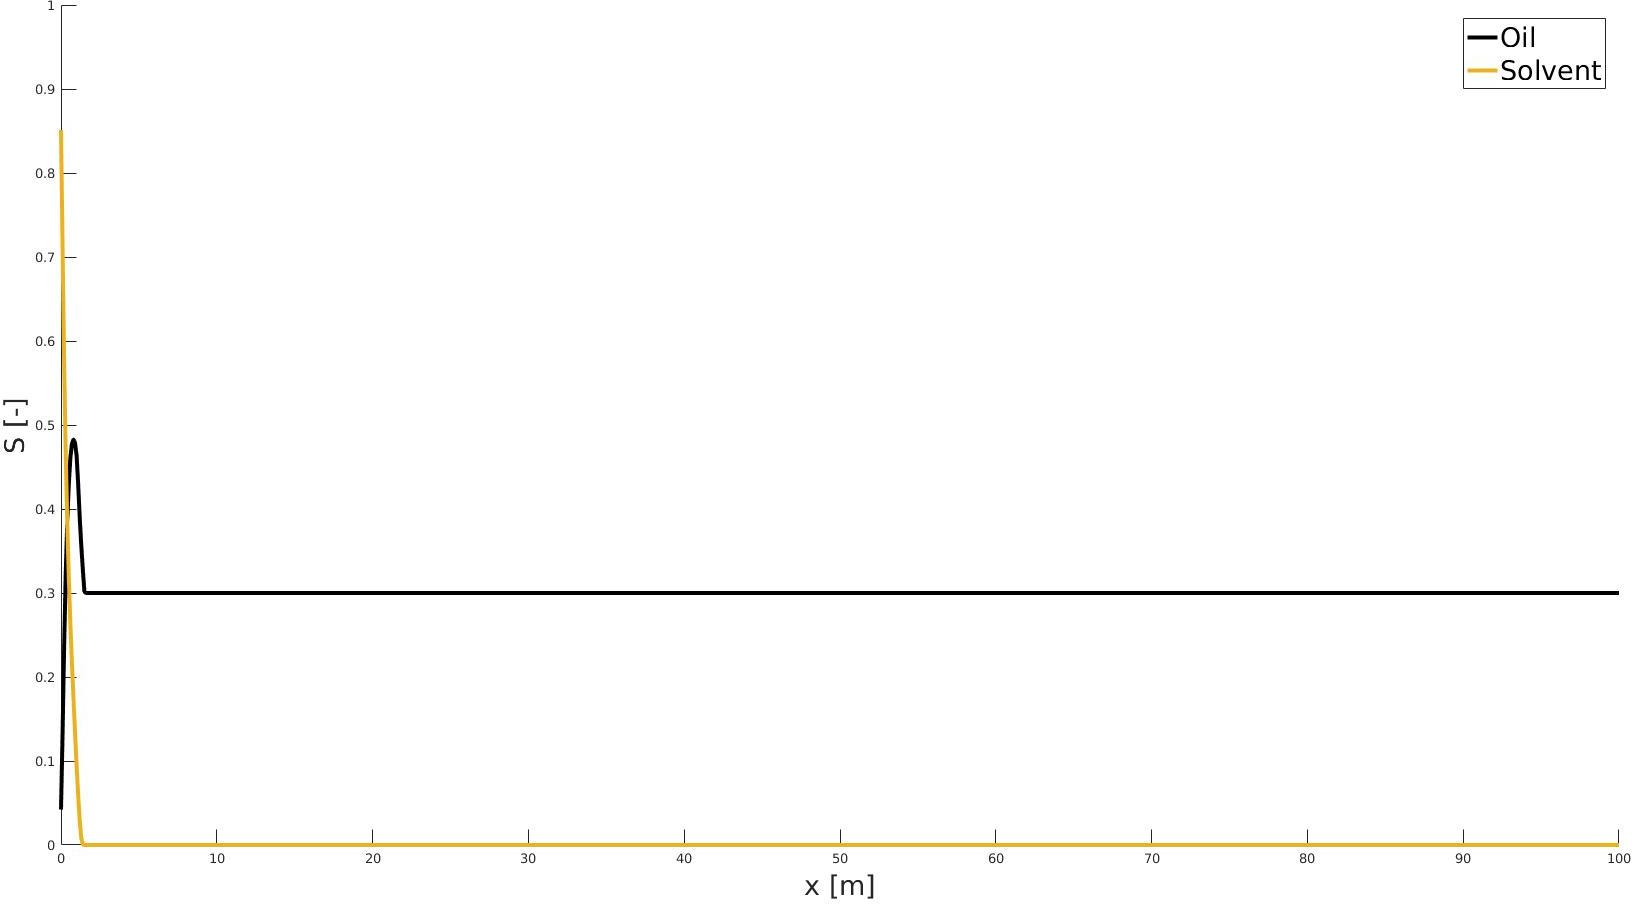
\includegraphics[width = 0.9\textwidth]{figures/displacement1D/displacement1Dplaceholder}}
    {figures/displacement1D/displacement1D.avi}
    \end{center}
  \end{mybox}
\end{frame}

\begin{frame}
  \frametitle{Example 2: Layer of SPE10}
  \begin{columns}
    \begin{column}{0.55\textwidth}
      \begin{itemize}
      \item Layer 10 of SPE10 model 2
      \item Initial saturation: $S_o = S_{or,i} = 0.3$, $S_w = 1 - S_{or, i}$
      \item Injection schedule: 1 Y waterflooding, 1 Y of 10 WAG cycles, 1 Y waterfloowing
      \end{itemize}
    \end{column}
    \begin{column}{0.45\textwidth}
      \begin{figure}[h]
        \centering
        \subfloat[Permeability]{
          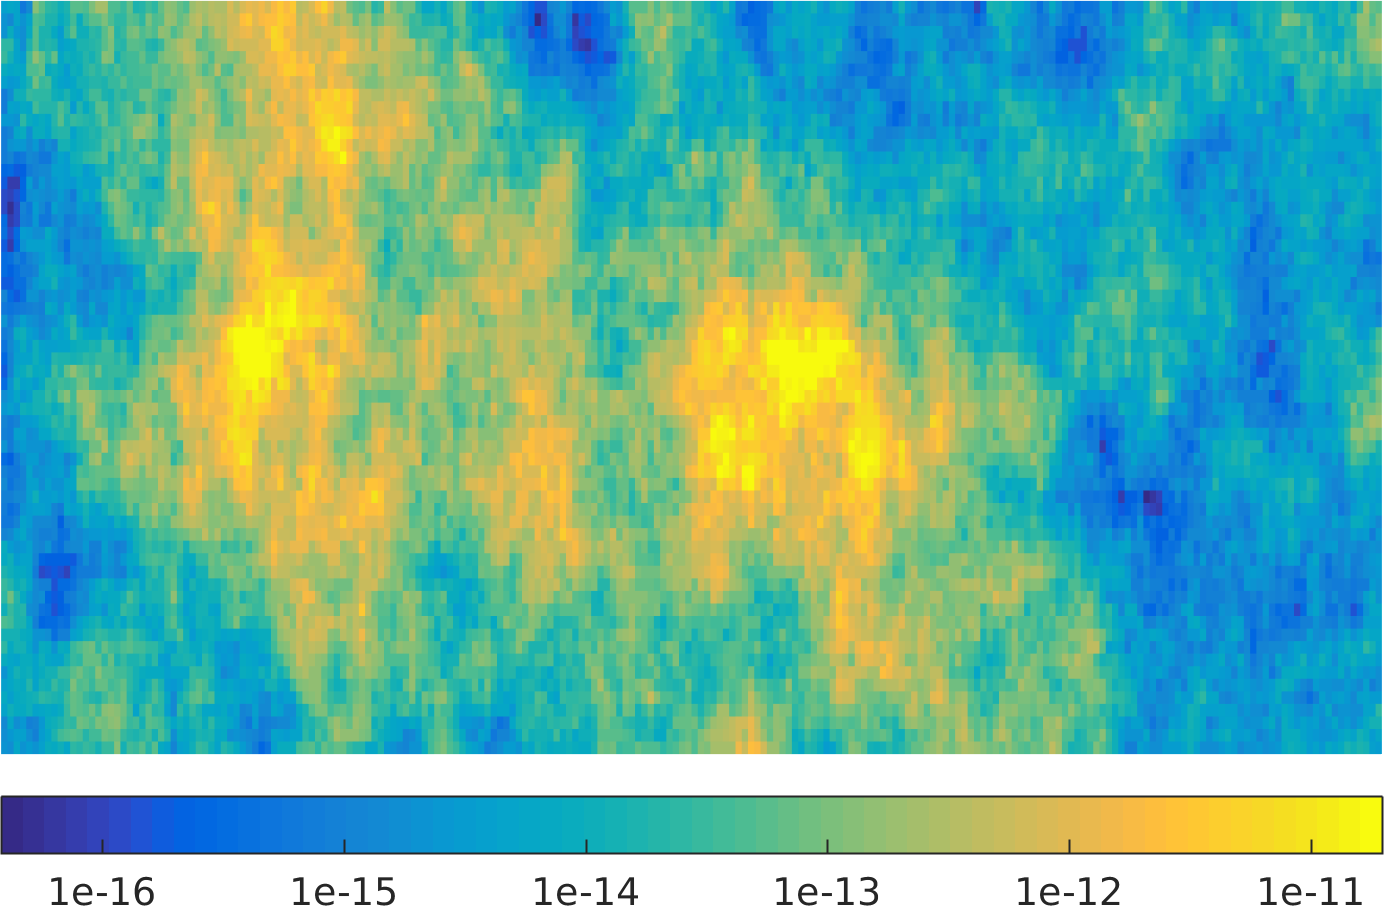
\includegraphics[width = 0.7\textwidth]{figures/spe10/spe10perm}} \\
        \subfloat[Porosity]{
          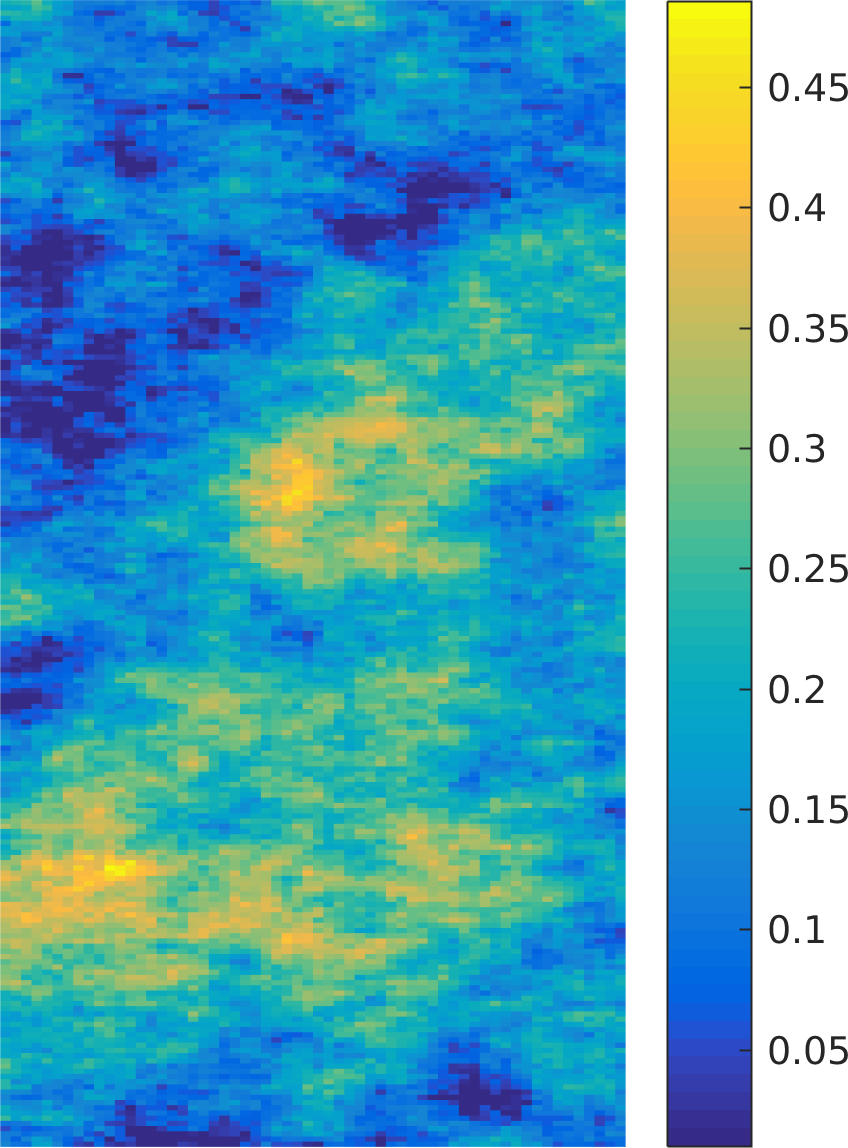
\includegraphics[width = 0.7\textwidth]{figures/spe10/spe10poro}}
      \end{figure}
    \end{column}
  \end{columns}
\end{frame}

\begin{frame}
  \frametitle{Example 1: 1D displacement}
  \centering
  \begin{mybox}{}{0.6\textheight}
    \begin{center}
    \movie[width = 1\textwidth]{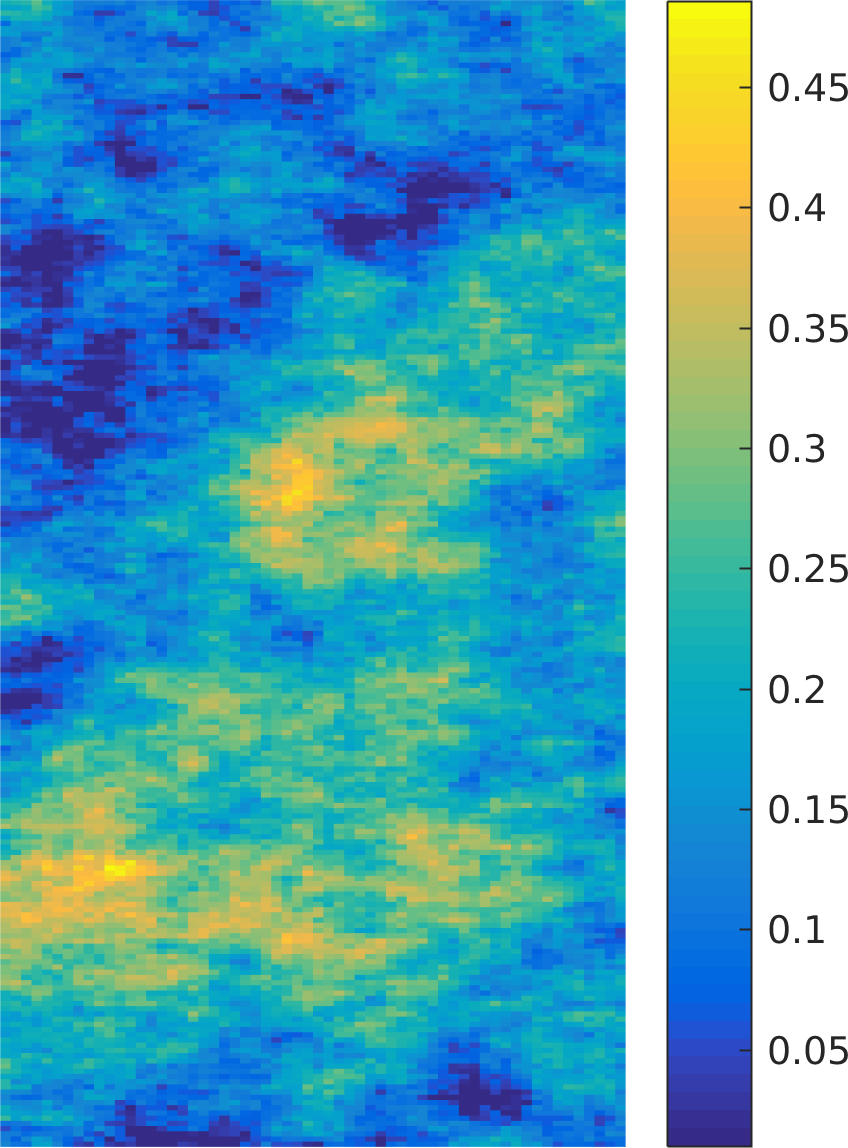
\includegraphics[width = 0.9\textwidth]{figures/spe10/spe10poro}}
    {figures/spe10/spe10.avi}
    \end{center}
  \end{mybox}
\end{frame}




\begin{frame}
  \frametitle{Example 2: Norne field model}
  
\end{frame}


\end{document}


%%% Local Variables:
%%% mode: latex
%%% TeX-master: t
%%% End:
